
\documentclass[10pt]{extarticle}
\usepackage[utf8]{inputenc}     % permite edição direta com acentos
\usepackage[pdftex]{hyperref}
\usepackage[margin=0.5in]{geometry}
\usepackage{fancyvrb}
\usepackage{graphicx}
\usepackage{listings}
\usepackage{color}

% PDF metadata
\hypersetup{
  pdfauthor={Lucas Brasilino and Sirshak Das},
  pdftitle={Computer Network Assignment 3 Write-up},
  pdfsubject={Computer Network},
  pdfkeywords={{Lucas Brasilino}, {Sirshak Das}},
  colorlinks=true,
  urlcolor=blue,
  linkcolor=black
}

% listings
\definecolor{listinggray}{gray}{0.9}
\definecolor{lbcolor}{rgb}{0.9,0.9,0.9}
\lstset{
	backgroundcolor=\color{lbcolor},
	tabsize=4,
	rulecolor=,
	language=C,
        basicstyle=\scriptsize\ttfamily,
        upquote=true,
        aboveskip={1.5\baselineskip},
        columns=fixed,
        showstringspaces=false,
        extendedchars=true,
        breaklines=true,
        prebreak = \raisebox{0ex}[0ex][0ex]{\ensuremath{\hookleftarrow}},
        frame=single,
        showtabs=false,
        showspaces=false,
        showstringspaces=false,
        identifierstyle=\ttfamily,
        keywordstyle=\color[rgb]{0,0,1},
        commentstyle=\color[rgb]{0.133,0.545,0.133},
        stringstyle=\color[rgb]{0.627,0.126,0.941},
}

% brackets around options
\newcommand{\abracket}[1]{$\langle$\texttt{#1}$\rangle$}
\newcommand{\specialcell}[2][c]{%
  \begin{tabular}[#1]{@{}c@{}}#2\end{tabular}}

\title{Computer Network Assignment 3 Write-up}
\author{Lucas Brasilino \\ 
  \href{mailto:lbrasili@indiana.edu}{lbrasili@indiana.edu}
  \and Sirshak Das\footnote{Names placed in alphabetical order} \\  
  \href{mailto:sirdas@indiana.edu}{sirdas@indiana.edu}
}
\date{}
\begin{document}                                 
\thispagestyle{empty}
\maketitle
%\centerline{\Large\textbf{Computer Network Assignment 3 Write-up}}   
%\vspace{0.1in}
%\centerline{\large{Lucas Brasilino and Sirshak Das}\footnote{Names placed in
%    alphabetical order}}
%\centerline{\texttt{\href{mailto:lbrasili@indiana.edu}{lbrasili@indiana.edu}}}
%\vspace{0.01in}

\section{Introduction}

The third programming assignment from P358 Computer Networks class is to
implement a Distance Vector routing. Each node, which are routers, has to send
their cost for reaching all nodes within the network to its immediate
neighbors. 

The resulting  Routing Information Protocol  (RIP) service from  this assignment
might support  update messages. These messages  might be sent in  a periodic and
asynchronous\footnote{As soon as  there is some routing table  update} ways. The
protocol is  well defined in  Figure~\ref{fig:protocol} and must use  UDP. After
receiving         update          messages,         a          node         uses
\href{https://en.wikipedia.org/wiki/Bellman%E2%80%93Ford_algorithm}{Bellman-Ford
Algorithm} to update its routing table. Finally,  if a node updates any costs in
its table, it sends an update message to its immediate neighbors.

\begin{figure}[!h]
\centering
\begin{BVerbatim}

                           32 bits
+--------------------------------------------------------------+
|                       IP address (4 bytes)                   |
+--------------------------------------------------------------+
|                          cost (4 bytes)                      |
+--------------------------------------------------------------+ 
|                       IP address (4 bytes)                   |
+--------------------------------------------------------------+
|                          cost (4 bytes)                      |
+--------------------------------------------------------------+
                             ...
\end{BVerbatim}
\caption{Update message}
\label{fig:protocol}
\end{figure}

\section{Implementation}

The developed program, called \texttt{rip}, was written in C using a private
repository in IU's GitHub server. It is organized in 3 directories:

\begin{itemize}
\item{\texttt{src}:} stores the source code files (\texttt{*.c})
\item{\texttt{include}:} stores the header files (\texttt{*.h})
\item{\texttt{test}:} stores sets of configuration files (\texttt{*.conf})
\end{itemize}

Some design decisions were made for \texttt{rip} development. First, it is a
multithreaded application. Second, internally not only node's IP addresses are
stored and manipulated, but also the node's hostname. This fact enables more
flexibility on the configuration file and better routing table
printouts. Finally, the functions in source code follows the convention
\texttt{rip\_<file>\_<name>()}, are organized in such a way that 
functions starting with \texttt{rip\_<file>\_*()} are placed in \texttt{rip\_<file>.c}
and each filename embed its purpose, as described bellow:
\begin{itemize}
\item{\texttt{rip\_main.c}:} It is the application entry point (function
  \texttt{main()}) and the main process. Also contains routines for parsing the
  command line arguments and configuration file, for the distance vector
  graph initialization and for running the mainloop. 
\item{\texttt{rip\_net.c}:} Encompass all network API, including the
  \textbf{send\_advertisement} component
  (\texttt{rip\_net\_send\_advertisement()}).
\item{\texttt{rip\_obj.c}:} This file contains all memory allocation
  deallocation functions for creating objects, like node information, route
  table entries, and protocol message entries.
\item{\texttt{rip\_routing.c}:} This file contains all the routing APIs including filling up of graph structure, distance vector and routing table.   
\item{\texttt{rip\_up.c}:} Contains the entry points for the other two threads:
  \textbf{rip\_up} and \textbf{rip\_up\_ttl}.
\end{itemize}

\section{Compilation}

On top directory a \texttt{Makefile} is provided for a easy compilation. As
expected, packages like gcc, make and glibc-dev must be installed in the Linux
system.

\begin{Verbatim}
$ make clean && make
\end{Verbatim}
%$

At the end of compilation process, the \texttt{rip} binary will be available in
this directory.

\section{Running the code}

In order to rule the application's behavior,  a set of command line options were
defined.          We           have          used           the          GlibC's
\href{http://www.gnu.org/software/libc/manual/html_node/Getopt.html}{getopt} API
to accomplish this functionality. The options are:

\begin{itemize}
\item{\texttt{-c}} \abracket{config\_file} : points to config file
\item{\texttt{-i}} \abracket{interface} : inform  by which interface the process
will bind to. The IP of it is also used as a identifier within the routing table
(array \texttt{routingtable[]}) (Default: eth0)
\item{\texttt{-u}} \abracket{port} : inform  which UDP port  might be  used for
receiving update messages
\item{\texttt{-p}} \abracket{period} : period,  in seconds, for  sending update
messages. (Default: 30)
\item{\texttt{-t}}  \abracket{ttl} :  the  expiration TTL  from  routing  table
(Default 3).  The final TTL  in seconds  is calculated by  period x ttl,  so the
default TTL, in seconds, is (3 x 30 = 90)
\item{\texttt{-y}}  \abracket{infinity} : set the infinity value (Default: 16)
\item{\texttt{-s}} : enables split horizon
\item{\texttt{-d}} : enables  debug, so the \texttt{stderr} is  sent to console,
otherwise it will be sent to file 'rip\_\abracket{hostname}.log'
\end{itemize}

\section{Configuration file format}

The configuration file follows exactly the formatting proposed by the
assignment. The first column is a node identifier, which can be an IP address or
its valid FQDN. In this context, \emph{valid FQDN} means that it can be resolved
using DNS or \texttt{/etc/hosts}.

Figures~\ref{fig:ipconf} and~\ref{fig:fqdnconf} shows examples of configuration files.
\begin{figure*}[!h]
\begin{minipage}[t]{0.4\textwidth}
\begin{Verbatim}[frame=single,framesep=10mm]
192.168.1.2 yes
192.168.1.3 yes
192.168.1.4 no
\end{Verbatim}
\caption{IP-based configuration file}
\label{fig:ipconf}
\end{minipage}
\hfill
\begin{minipage}[t]{0.4\textwidth}
\begin{Verbatim}[frame=single,framesep=10mm]
basalt.soic.indiana.edu yes
blesmol.soic.indiana.edu no
bobac.soic.indiana.edu yes
\end{Verbatim}
\caption{FQDN-based configuration file}
\label{fig:fqdnconf}
\end{minipage}
\end{figure*}

\newpage
\section{Application Internals}

This section documents all application internals aspects.

\subsection{Principal data structures}

The very basic data structure is the \texttt{node\_info\_t}. It holds the FQDN
name of the node and its IP address in a \texttt{struct sockaddr\_in}
structure.

\begin{lstlisting}
/**
 * Information about nodes (to be used in graph/table)
 * 
 */
struct _node_info
{
    char *name;			/**< Name of the node */
    struct sockaddr_in *inet;	/**< Inet related information */
};

typedef struct _node_info *node_info_t;
\end{lstlisting}

The \texttt{route\_entry\_t} data structure uses the \texttt{node\_info\_t}
information to maintain a routing table entry. The route table itself is the
\texttt{routingtable[]} array. The global variable
\texttt{rip\_routing\_table\_entry\_number} register the number of entries in the
routing table.

\begin{lstlisting}
/**
 * Route entry for routing table
 * 
 */
struct _route_entry
{
    node_info_t destination;	/**< Destination */
    node_info_t nexthop;	/**< Next hop */
    cost_t cost;		/**< Cost */
    unsigned short int ttl;	/**< TTL */
};

typedef struct _route_entry *route_entry_t;

unsigned int rip_routing_table_entry_number;
route_entry_t routingtable[MAXROUTE];
\end{lstlisting}

As will be described later, the \texttt{rip} application uses a data structure
called \texttt{adtable} to pass the advertised table received by the main thread
(from a node) to the \textbf{rip\_up} thread in order to do routing
calculations. So, this data structure is type \texttt{advert\_entry\_t}:

\begin{lstlisting}
/**
 * Advertisement received from neighbor. This struct is 
 * populated from message. advert_entry_t is not a pointer
 */
struct _advert_entry
{
    node_info_t neighbor;		/**< Advertisement sender */
    route_entry_t neightable[MAXROUTE]; /**< Advertised table */
    bool_t ready;                       /**< Advertised message ready for thread*/
    bool_t is_empty;                    /*is advent_entry buff empty*/
};

typedef struct _advert_entry advert_entry_t;

advert_entry_t adtable;
\end{lstlisting}

The UDP message itself must be in the form as depicted in
Figure~\ref{fig:protocol}. To accomplish this the type
\texttt{message\_entry\_t} has two fiels: dest\_addr and cost, both 4 bytes legth.

\begin{lstlisting}
/**
 * Each entry of a message. 
 * It is not a pointer because its desirable to be in-memory aligned.
 */
struct _message_entry 
{
    struct in_addr dest_addr;
    cost_t cost;
};

typedef struct _message_entry message_entry_t;
\end{lstlisting}

\newpage
The graph is implemented by \texttt{r\_graph}, which is an adjacency table: 
2 dimensional array, where each element has \texttt{cost} and \texttt{ttl} information.

\begin{lstlisting}
typedef struct _route_graph_entry
{
    cost_t             cost;
    unsigned short int ttl;
} route_graph_entry_t;

typedef route_graph_entry_t*  route_graph_row_t;
typedef route_graph_entry_t** route_graph_t;
route_graph_t r_graph;
\end{lstlisting}

Finally, the  distance vector is maintainend  in \texttt{dist\_hop\_vect}, which
is   typed    as   \texttt{route\_dist\_hop\_vect\_t},   as   an    array   with
\texttt{hop\_index}  and \texttt{cost}.  \texttt{hop\_index} is  the index  of the
nexthop node present the same array. This  index is used to fill in the next\_hop
node details in  the routing table. This is  an index used also in  the rows and
columns in the graph.

\begin{lstlisting}
typedef struct _route_dist_hop
{
    cost_t       cost;
    unsigned int hop_index;
} route_dist_hop_t;
typedef route_dist_hop_t* route_dist_hop_vect_t;

route_dist_hop_vect_t dist_hop_vect;
\end{lstlisting}

\subsection{Main process and threads}

The \texttt{rip} application runs a main process and spawns 2 threads:
\textbf{rip\_up} and \textbf{rip\_up\_ttl}.

\paragraph{The main  process} It  parses the command  line options,  parses the
config file, builds the initial routing  table, starts to listen to UDP messages
and spawns the \textbf{rip\_up} and \textbf{rip\_up\_ttl} threads. After that, it enters
in  a   infinite  loop  (\texttt{rip\_main\_loop()})  listen   to  other's  node
advertisements   (\texttt{rip\_net\_recv\_advertisement()})   and   passes   the
received              information               to              \textbf{rip\_up}
(\texttt{rip\_obj\_push\_recv\_advertisement()}) using the \texttt{adtable} data
structure, using \texttt{lock} mutex for synchonization.

\paragraph{rip\_up}  This thread  retrieves the  message received  by the  main
thread  and fill  the  advertised  route into  the  graph  structure. Then  runs
Bellman-Ford (\texttt{rip\_routing\_bellman\_ford()}) on the graph which relaxes
all the edges and computes  the distance vector hold on \texttt{dist\_hop\_vect}
data  structure.   This is  a   scaled  down  version   of  the
\texttt{routingtable[]}, i.e, it only contains the nexthop as hop\_index and the
cost.   Ttl is  determined from  the graph  or from  the message  received. Once
Bellman-Ford computes  the distance  vector, this  thread compares  the distance
vector to  the routing  table. If  the there is  a change  and sends  a triggered
update immediately.  If not, it  checks for the last  time when last  update was
send and,  if a periodic update  is required, it sends  accordingly. This thread
also  calculates the  Convergence Time,  by  calculating the  time elapsed  from
\texttt{start\_time}  to   the  time   when  no  updates   force  a   change  in
\texttt{routingtable[]}. When it  occurs, the thread updates  the start\_time to
the new time. This thread uses 2 mutexes: \texttt{lock} and \texttt{graph\_lock}.
The  former  for  accessing  \texttt{adtable}   and  the  latter  for  accessing
\texttt{r\_graph}. It shares the first mutex with main process and the second one
with \textbf{rip\_up\_ttl} thread.

\paragraph{rip\_up\_ttl}: This thread sleeps for period time (defined by the
\texttt{-p} option), wakes up, executes a procedure, and then goes back to sleep
again. The procedure is to decrease the ttl value in each graph node and if ttl
value reaches 0 it sets the COST to \texttt{COST\_INFINITY} (16). 
It uses the mutex \texttt{graph\_lock} to synchronize access to shared data
structure \texttt{r\_graph}.

\subsection{Global, shared, conditional variables and mutexes}

In the application implementation, all global variables are also shared at least
between the main process and the thread \textbf{rip\_up}. They are:

\begin{itemize}
\item{\texttt{routingtable}:} the routing table array;
\item{\texttt{rip\_routing\_table\_entry\_number}:} the quantity of entries in
  routing table;
\item{\texttt{adtable}:} the advertised table received from a neighbor;
\item{\texttt{r\_graph}:} the graph, i.e., the cost and ttl to a given
  node. Each index is associated with the index in the routing table;
\end{itemize}

The conditional variables are members of \texttt{adtable} data structure. They are:

\begin{itemize}
\item{\texttt{adtable.ready}:} Is used by the main process to signals
  \textbf{rip\_up} thread that it must execute;
\item{\texttt{adtable.is\_empty}:} Tells \textbf{rip\_up} thread if
  \texttt{adtable} is empty. If it is empty, \textbf{rip\_up} checks if sending update
is required (\texttt{rip\_util\_is\_update\_required()}). If the result is true, 
\texttt{rip\_net\_send\_advertisement()} is called. If \texttt{adtable} is not
empty,
i.e., the node has received an advertisement message, it calculates and updates
the distance vector and the graph.
\end{itemize}

\subsection{Mutexes}

Two mutexes are used in the application:

\begin{lstlisting}
/* Mutex */
pthread_mutex_t lock;
pthread_mutex_t graph_lock;
\end{lstlisting}

\texttt{lock} mutex controls the access to \texttt{adtable} between the main
process and \textbf{rip\_up} thread. \texttt{graph\_lock} mutex controls the
access to \texttt{r\_graph} between \textbf{rip\_up} and \textbf{rip\_up\_ttl}
threads.

\section{Test cases}

For application evaluation, some test cases were designed and performed.

\subsection{Test Case 1}

In this test case, three nodes were executed in a linear topology as depicted in
Figure~\ref{fig:testcase1}. Table~\ref{tab:testcase1nosh} shows the convergence
time without using split horizon, while Table~\ref{tab:testcase1sh} shows the
results with split horizon. In both tables the results are grouped by
parenthesis, but each value correspond to a node. Finally, all times are in
seconds, including Infinity and Period.

\begin{figure}[!h]
  \centering
    
\includegraphics[scale=0.50]{TestCase1.png}
    \caption{Test Case 1 three nodes linear topology}
    \label{fig:testcase1}
\end{figure}

\begin{table}[h]
\caption{Convergence time without split horizon}
\label{tab:testcase1nosh}
\centering
\begin{tabular}{| c | c | c | c |}
\hline
Infinity & Period & \specialcell{Initialization\\(node 1, node 2, node 3)}  &
\specialcell{One down\\(node 1, node 2)} \\
\hline
\hline
16 & 10 & (20, 9, 17) & (40, 60) \\
16 & 30 & (61, 29, 54) & (90, 150) \\
50 & 10 & (20, 9, 18) & (30, 50) \\
50 & 30 & (60, 29, 57) & (90, 150)\\
\hline
\end{tabular}
\end{table}

\begin{table}[h]
\caption{Convergence time with split horizon}
\label{tab:testcase1sh}
\centering
\begin{tabular}{| c | c | c | c | c | c | c |}
\hline
Infinity & Period & \specialcell{Initialization\\(node 1, node 2, node 3)}  &
\specialcell{One down\\(node 1, node 2)} \\
\hline
\hline
16 & 10 & (20, 9, 18)  & (40, 40) \\
16 & 30 & (60, 29, 57)  & (120, 120) \\
50 & 10 & (20, 8, 16) & (40, 40) \\
50 & 30 & (60, 29, 57)  & (120, 120) \\
\hline
\end{tabular}
\end{table}

One thing we observed was that with split horizon we get better convergence time
than without in case of one node  failure(120 - With split horizon 150 - without
split  horizon). There  is no  visible difference  in convergence  time in  case
intitialization.  Similar  trend is  observed when  we vary  the period  from 30
seconds to 10 seconds.

\newpage

\subsection{Test Case 2}

In this test case, four nodes were executed in a cyclic topology as depicted in
Figure~\ref{fig:testcase2}. Again, Table~\ref{tab:testcase2nosh} shows the convergence
time without using split horizon, while Table~\ref{tab:testcase2sh} shows the
results with split horizon.

\begin{figure}[!h]
  \centering
    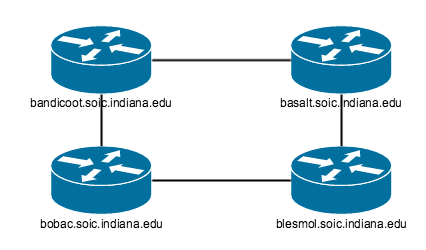
\includegraphics[scale=0.50]{TestCase2.png}
    \caption{Test Case 2 four nodes cyclic topology}
    \label{fig:testcase2}
\end{figure}

\begin{table}[h]
\caption{Convergence time without split horizon}
\label{tab:testcase2nosh}
\centering
\begin{tabular}{| c | c | c | c |}
\hline
Infinity & Period & \specialcell{Initialization\\(node 1, node 2, node 3, node 4)}  &
\specialcell{One down\\(node 1, node 2, node 4)} \\
\hline
\hline
16 & 10 &  (20, 10, 19, 9) & (338, 30, 30) \\
16 & 30 &  (60, 28, 56, 25) & (1947, 387, 390) \\
50 & 10 &  (20, 9, 18, 7) &  (616, 30, 30) \\
50 & 30 &  (60, 28, 56, 24) & (3528, 392, 390) \\
\hline
\end{tabular}
\end{table}

\begin{table}[h]
\caption{Convergence time with split horizon}
\label{tab:testcase2sh}
\centering
\begin{tabular}{| c | c | c | c |}
\hline
Infinity & Period & \specialcell{Initialization\\(node 1, node 2, node 3, node 4)}  &
\specialcell{One down\\(node 1, node 2, node 4)} \\
\hline
\hline
16 & 10 & (20, 8, 17, 7)  & (30, 30, 40) \\
16 & 30 & (60, 28, 57, 26)  & (90, 90, 120)  \\
50 & 10 & (10, 9, 8, 8)  & (20, 20, 41) \\
50 & 30 &  (30, 27, 25, 24)  & (60, 60, 120) \\
\hline
\end{tabular}
\end{table}

Confirming our  observation from  the previous  test case here  also we  see the
convergence time without  split horizon being very high compared  to low in case
of split horizon(With  split horizon: 120 Without Split Horizon:  1947). One new
trend which we observed  in this test case was the  variance in convergence time
without  split horizon  when  we vary  the INFINITY  COST(INFINITY:  16 -  Time:
1947,INFINITY: 50  Time: 3528). Again  this trend is the  same when we  vary the
period from 30 to 10 seconds.

\end{document}

